\section{Buscador}

A diferencia del indexador, la aplicación del buscador sí que dispone de interfaz gráfica, permitiendo al usuario realizar múltiples consultas sobre el índice de manera sencilla en una misma sesión. Para construir esta interfaz, se ha usado \textbf{JavaFX}, obteniendo el resultado siguiente:

\begin{figure}[H]
    \centering
    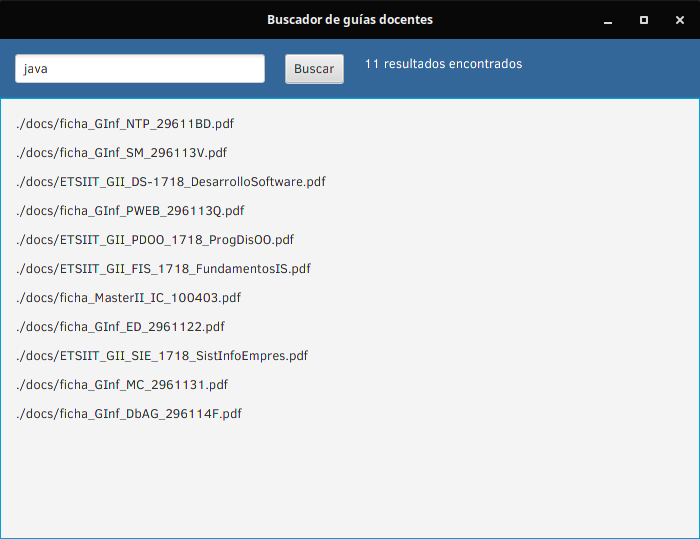
\includegraphics[width=1\linewidth]{images/searcher-ui.png}
\end{figure}

Para realizar las búsquedas, se necesitan tanto un \verb|QueryParser| para interpretar las consultas (con el mismo procedimiento usado para procesar los documentos) como un \verb|IndexSearcher| para realizar las búsquedas como tal sobre el índice. Estos objetos se construyen así:

\begin{lstlisting}[language=Java]
private IndexSearcher createIndexSearcher(Path indexPath) {
    IndexSearcher searcher = null;

    try {
        Directory indexDir = FSDirectory.open(indexPath);
        IndexReader reader = DirectoryReader.open(indexDir);
        searcher = new IndexSearcher(reader);
    } catch (IOException e) {
        System.out.println("Can't create index searcher - Error: " + e.getMessage());
        System.exit(1);
    }

    return searcher;
}

private QueryParser createQueryParser(Path stopwordsPath) {
    QueryParser parser = null;

    try {
        // Read stopwords from file
        var stopwords = readStopwords(stopwordsPath);

        // Create parser
        Analyzer analyzer = new SpanishAnalyzer(new CharArraySet(stopwords, true));
        parser = new QueryParser("contents", analyzer);
    } catch (IOException e) {
        System.out.println("Can't create query parser - Error: " + e.getMessage());
        System.exit(1);
    }

    return parser;
}
\end{lstlisting}

Una vez hecho esto, creamos la interfaz, dotando al botón de la funcionalidad de búsqueda, la cuál se puede ver a continuación:

\begin{lstlisting}
// Search button
Button searchBtn = new Button("Buscar");
searchBtn.setOnAction(new EventHandler<ActionEvent>() {

    @Override
    public void handle(ActionEvent e) {
        msgLabel.setText("");

        String inputString = queryTF.getText();
        if (inputString.isEmpty()) {
            msgLabel.setText("Por favor, introduce un termino para la busqueda");
            return;
        }

        try {
            Query query = parser.parse(inputString);
            var results = indexSearcher.search(query, 50).scoreDocs;
            resultsPane.refresh(results);
            msgLabel.setText(results.length +" resultados encontrados");
        } catch (ParseException pe) {
            msgLabel.setText("No se ha podido procesar la consulta");
        } catch (IOException ioe) {
            msgLabel.setText("Error en la consulta del indice");
        }
    }
});
\end{lstlisting}

Como su propio nombre indica, \verb|resultsPane| es el panel de la interfaz en el que se muestran los resultados. Llamando a su método \verb|refresh| con los nuevos resultados, lo que hacemos es refrescar el panel para mostrarlos. La construcción de los resultados en la interfaz se puede ver a continuación:

\begin{lstlisting}[language=Java]
public void refresh(ScoreDoc[] results) {
    this.getChildren().clear();

    for (int i = 0; i < results.length; i++) {
        try {
            Document doc = indexSearcher.doc(results[i].doc);
            this.getChildren().add(buildResult(doc));
        } catch (IOException e) {
            System.out.println("Can't retrieve result - Error: " + e.getMessage());
        }
    }
}

private HBox buildResult(Document doc) {
    HBox box = new HBox();
    box.setSpacing(15.0);

    // Add label with doc path
    Label pathLabel = new Label(doc.get("path"));
    box.getChildren().add(pathLabel);

    return box;
}
\end{lstlisting}

\subsection{Manual de uso}

Para lanzar la aplicación del buscador, debemos ejecutar el archivo \verb|jar| desde la línea de comandos, indicando las rutas al índice y al archivo de palabras vacías, de esta manera:

\begin{lstlisting}
java -jar searcher.jar --stopwords=[Ruta a fichero] --index=[Ruta a indice]
\end{lstlisting}

Una vez en la interfaz, para realizar una búsqueda sólo debe introducir los términos de la misma en el campo de texto y pulsar sobre el botón "Buscar".